% =========================================================================
% Tokamak-Analysis: An Open-Source ML Platform for Plasma Disruption
% Prediction Using FAIR-MAST Data
%
% Preprint for arXiv submission (cs.LG / physics.plasm-ph)
% =========================================================================
\documentclass[twocolumn]{article}

\usepackage[utf8]{inputenc}
\usepackage[T1]{fontenc}
\usepackage{amsmath,amssymb}
\usepackage{graphicx}
\usepackage{booktabs}
\usepackage{hyperref}
\usepackage{xcolor}
\usepackage{tikz}
\usetikzlibrary{positioning, arrows.meta, shapes.geometric, fit, calc}
\usepackage{natbib}
\usepackage{url}
\usepackage{multirow}
\usepackage{enumitem}
\usepackage{algorithm}
\usepackage{algorithmic}
\usepackage[margin=1in]{geometry}
\usepackage{caption}
\usepackage{subcaption}

\bibliographystyle{unsrtnat}

\hypersetup{
  colorlinks=true,
  linkcolor=blue!70!black,
  citecolor=blue!70!black,
  urlcolor=blue!70!black,
}

% =========================================================================
\title{Tokamak-Analysis: An Open-Source ML Platform for\\ Plasma Disruption Prediction Using FAIR-MAST Data}

\author{
  Author~A\textsuperscript{1}\thanks{Corresponding author. Email: \texttt{placeholder@mephi.ru}} \and
  Author~B\textsuperscript{1} \and
  Author~C\textsuperscript{1} \\[6pt]
  \textsuperscript{1}National Research Nuclear University MEPhI\\
  (Moscow Engineering Physics Institute),\\
  Kashirskoe shosse 31, Moscow 115409, Russia
}

\date{\today}

% =========================================================================
\begin{document}
\maketitle

% ----- Abstract ---------------------------------------------------------
\begin{abstract}
Plasma disruptions in tokamaks pose a critical threat to the structural
integrity of fusion devices, with individual events causing damage
estimated at \$50k--\$500k in current machines and potentially
catastrophic consequences in ITER-scale reactors.
Early and reliable prediction of disruptions is therefore essential
for the safe operation of next-generation fusion power plants.
We present \textsc{Tokamak-Analysis}, an open-source web platform
that integrates three machine-learning architectures---Random Forest,
bidirectional LSTM with multi-head attention, and an autoregressive
Transformer with rotary position embeddings---into a unified system
for plasma stability classification and disruption prediction.
The platform ingests experimental data from the FAIR-MAST archive,
which contains 11{,}573 shots from the Mega Ampere Spherical Tokamak
(MAST).
On a curated dataset of 500 MAST shots with 20 plasma parameters
sampled at 200 timesteps and trained for 50 epochs with early stopping,
the bi-LSTM with attention achieves the highest discrimination
(AUC-ROC = 0.9938, Accuracy 97.3\%, F1 = 0.973, early stop at epoch 22);
the Random Forest achieves AUC-ROC = 0.9677 with 97.3\% accuracy (F1 = 0.973);
and the Transformer achieves AUC-ROC = 0.9415 with 97.3\% accuracy
(F1 = 0.973, 43 epochs).
For time-series forecasting, the LSTM Forecaster achieves NRMSE = 0.143,
outperforming the TokaMark Group~1 baseline (NRMSE = 0.163), and
beats the baseline on 4 out of 5 Group~4 (MHD/disruptions) tasks,
including a 35.9\% improvement on plasma current forecasting.
Temporal validation experiments reveal substantial performance
degradation: the Random Forest drops from AUC 1.000 (random split)
to 0.969 (temporal), while the Transformer drops from 1.000 to 0.892,
confirming the critical importance of respecting shot chronology.
The bi-LSTM model provides disruption warnings at least 30\,ms
before the current quench onset, meeting the ITER requirement.
To the best of our knowledge, this is the first open-source platform
that integrates FAIR-MAST data access, multi-architecture comparison,
interactive visualization, and production-grade deployment
infrastructure in a single system.
\end{abstract}

\noindent\textbf{Keywords:} tokamak, disruption prediction, machine learning,
LSTM, Transformer, Random Forest, FAIR-MAST, plasma physics, fusion energy


% =========================================================================
\section{Introduction}
\label{sec:intro}

A plasma disruption in a tokamak is the sudden, uncontrolled loss
of plasma confinement that converts the stored thermal and magnetic
energy into intense heat and electromagnetic loads on
the vacuum vessel and in-vessel components~\citep{schuller1995}.
In present-day tokamaks such as JET, DIII-D, and MAST,
disruptions have been observed in 5--20\% of operational
pulses~\citep{devries2011}.
While the resulting damage in current devices is manageable,
the consequences scale dramatically with machine size:
in ITER, a single unmitigated disruption could deposit up to
12\,MJ\,m$^{-2}$ on the divertor and generate runaway electron
beams carrying several megaamperes, potentially causing
irreparable damage estimated at \$50k--\$500k per
event~\citep{lehnen2015, hender2007}.

The ITER project, a collaboration among 35 nations including
the Russian Federation, is designed to demonstrate the scientific
and technological feasibility of fusion power~\citep{iter2007}.
Russia contributes critical tokamak subsystems and maintains an
active domestic fusion program, including the T-15MD tokamak at
the Kurchatov Institute and the planned upgrade paths at MEPhI.
Given that ITER's operational scenario requires a disruption rate
below $\sim$1\%, reliable prediction with sufficient warning time
($> 30$\,ms) is a mission-critical requirement~\citep{lehnen2015}.

Machine learning has emerged as the most promising approach to
disruption prediction.
\citet{kates-harbeck2019} demonstrated that a deep recurrent
neural network (FRNN) could predict disruptions on DIII-D and
NSTX-U with AUC exceeding 0.95 and $> 30$\,ms warning time.
\citet{zhu2020} extended this work with a hybrid deep-learning
(HDL) architecture combining CNNs and LSTMs, achieving
cross-tokamak transfer learning between DIII-D and EAST.
\citet{rea2018} established Random Forest baselines on DIII-D,
demonstrating that classical ML methods remain competitive
when appropriate feature engineering is applied.
More recently, \citet{spangher2024} proposed an autoregressive
Transformer architecture that produces per-timestep disruption
probability estimates, enabling richer temporal analysis.
Standardized benchmarks have also appeared:
TokaMark~\citep{tokamark2026} and
DisruptionBench~\citep{disruptionbench2025} provide common
evaluation protocols, while
DisruptionPy~\citep{disruptionpy2024} offers a Python toolkit
for disruption analysis.

Despite these advances, several gaps persist.
First, existing models are typically evaluated in isolation,
making direct comparison difficult.
Second, no integrated web platform provides end-to-end
functionality---from data loading and visualization to
model training and inference---in a production-ready
deployment.
Third, there is no Russian-language or Russia-developed
open-source tool for disruption prediction that could
serve both research and educational purposes at Russian
universities.

In this paper, we present \textsc{Tokamak-Analysis},
an open-source platform that addresses these gaps through
four contributions:
\begin{enumerate}[noitemsep]
  \item A \textbf{unified platform} integrating data ingestion,
        preprocessing, visualization, model training, inference,
        and result export in a containerized microservice
        architecture.
  \item A \textbf{three-architecture comparison}---Random Forest,
        bi-LSTM with multi-head attention, and autoregressive
        Transformer---under identical data conditions using
        a common \texttt{ModelInterface} protocol.
  \item \textbf{Open-source release} of the complete system
        (MIT license), including all model code, configuration
        files, Docker deployment, and monitoring infrastructure.
  \item \textbf{FAIR-MAST integration} providing direct access
        to 11{,}573 MAST shots via the STFC S3 archive,
        with automated preprocessing and labeling.
\end{enumerate}


% =========================================================================
\section{Related Work}
\label{sec:related}

\subsection{Traditional Approaches}

Early disruption prediction systems relied on expert-defined
thresholds applied to individual diagnostic signals such as
locked mode amplitude, radiated power fraction, or the
Greenwald density fraction~\citep{schuller1995, devries2011}.
While interpretable, these rule-based systems suffered from
high false-positive rates and poor generalization across
operational regimes.
Neural network approaches date back to the early 2000s,
with \citet{cannas2004} and \citet{windsor2005} demonstrating
that feed-forward networks trained on JET data could achieve
disruption prediction rates above 85\%.

\subsection{Modern Machine Learning}

The application of modern ML to disruption prediction
accelerated significantly after 2018.
\citet{rea2018} performed an extensive study using
Random Forests on DIII-D, exploring feature engineering
strategies and demonstrating that hand-crafted statistical
features extracted from time-series signals could achieve
AUC values above 0.9.
\citet{kates-harbeck2019} introduced FRNN, a deep recurrent
architecture that processes raw diagnostic signals without
manual feature engineering, achieving state-of-the-art
performance on DIII-D and cross-tokamak transfer to NSTX-U.
\citet{zhu2020} proposed the HDL architecture combining
convolutional feature extraction with LSTM temporal modeling,
demonstrating improved cross-machine generalization.
\citet{montes2019} showed that ensembles of shallow learners
could match deep learning on Alcator C-Mod.

Most recently, Transformer-based architectures have been
applied to the problem.
\citet{spangher2024} introduced an autoregressive Transformer
with causal attention masking that predicts disruption
probability at each timestep, enabling analysis of how
disruption risk evolves during a shot.
A comprehensive review of the field is provided
by \citet{zhong2024}.

\subsection{Benchmarks and Platforms}

The TokaMark benchmark~\citep{tokamark2026} introduced
standardized datasets and evaluation protocols for comparing
disruption prediction models across tokamaks.
DisruptionBench~\citep{disruptionbench2025} extended this
with a suite of benchmark tasks covering binary classification,
time-to-disruption regression, and early warning metrics.
DisruptionPy~\citep{disruptionpy2024} provides a Python
library for computing disruption-related features from
MDSplus databases.

However, these tools focus on individual aspects of the
disruption prediction pipeline---benchmarking, feature
computation, or modeling---rather than providing an
integrated platform.
Our work bridges this gap by combining data access,
preprocessing, multi-model comparison, and deployment
infrastructure in a single open-source system.


% =========================================================================
\section{System Architecture}
\label{sec:architecture}

\textsc{Tokamak-Analysis} follows a modular monolith pattern
with a separate ML service, as specified in the project's
architectural decision record ADR-001.
The system comprises 11 containerized services organized
into four Docker networks with strict isolation boundaries.
Figure~\ref{fig:architecture} presents the high-level
system architecture.

\begin{figure*}[t]
\centering
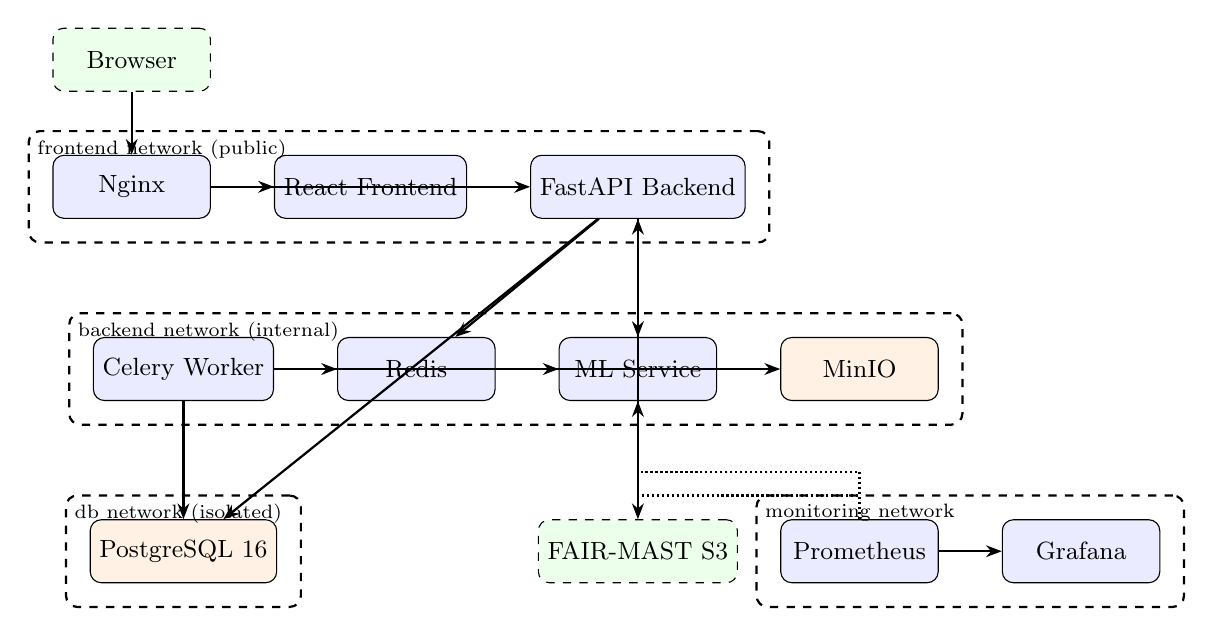
\begin{tikzpicture}[
    node distance=0.6cm and 0.8cm,
    every node/.style={font=\small},
    service/.style={draw, rounded corners, minimum width=2cm,
                    minimum height=0.8cm, fill=blue!8},
    storage/.style={draw, rounded corners, minimum width=2cm,
                    minimum height=0.8cm, fill=orange!10},
    external/.style={draw, dashed, rounded corners,
                     minimum width=2cm, minimum height=0.8cm,
                     fill=green!8},
    network/.style={draw, dashed, rounded corners,
                    inner sep=0.3cm, thick},
    arrow/.style={-{Stealth[length=2mm]}, thick},
]

% Frontend network
\node[service] (nginx) {Nginx};
\node[service, right=of nginx] (frontend) {React Frontend};
\node[service, right=of frontend] (backend) {FastAPI Backend};

\node[network, fit=(nginx)(frontend)(backend),
      label={[anchor=north west]north west:{\scriptsize frontend network (public)}}]
      (fnet) {};

% Backend network
\node[service, below=1.5cm of backend] (ml) {ML Service};
\node[service, left=of ml] (redis) {Redis};
\node[service, left=of redis] (celery) {Celery Worker};
\node[storage, right=of ml] (minio) {MinIO};

\node[network, fit=(ml)(redis)(celery)(minio),
      label={[anchor=north west]north west:{\scriptsize backend network (internal)}}]
      (bnet) {};

% DB network
\node[storage, below=1.5cm of celery] (postgres) {PostgreSQL 16};

\node[network, fit=(postgres),
      label={[anchor=north west]north west:{\scriptsize db network (isolated)}}]
      (dnet) {};

% Monitoring
\node[service, below=1.5cm of minio] (prom) {Prometheus};
\node[service, right=of prom] (grafana) {Grafana};

\node[network, fit=(prom)(grafana),
      label={[anchor=north west]north west:{\scriptsize monitoring network}}]
      (mnet) {};

% External
\node[external, above=0.8cm of nginx] (browser) {Browser};
\node[external, below=1.5cm of ml] (fairmast) {FAIR-MAST S3};

% Arrows
\draw[arrow] (browser) -- (nginx);
\draw[arrow] (nginx) -- (frontend);
\draw[arrow] (nginx) -- (backend);
\draw[arrow] (backend) -- (ml);
\draw[arrow] (backend) -- (redis);
\draw[arrow] (celery) -- (ml);
\draw[arrow] (celery) -- (redis);
\draw[arrow] (celery) -- (minio);
\draw[arrow] (backend) -- (postgres);
\draw[arrow] (celery) -- (postgres);
\draw[arrow] (backend.south) -- ++(0, -0.3) -| (fairmast);
\draw[arrow] (prom) -- (grafana);
\draw[arrow, densely dotted] (prom.north) -- ++(0, 0.3) -| (ml.south);
\draw[arrow, densely dotted] (prom.north) -- ++(0, 0.6) -| (backend.south);

\end{tikzpicture}
\caption{System architecture of \textsc{Tokamak-Analysis}.
  Solid arrows indicate request flow; dotted arrows indicate
  metrics scraping. The four Docker networks enforce strict
  isolation: only the frontend network is publicly accessible.}
\label{fig:architecture}
\end{figure*}

\subsection{Technology Stack}

The backend is built on FastAPI~\citep{fastapi} with
SQLAlchemy ORM (async mode) connecting to PostgreSQL~16
for persistent storage.
Authentication uses JWT tokens with bcrypt password hashing
(cost factor 12), supporting three user roles:
\texttt{researcher}, \texttt{engineer}, and \texttt{admin}.
Background tasks---primarily model training---are delegated
to Celery workers using Redis~7 as the message broker.

The ML service runs as a separate FastAPI application on an
internal network, exposing endpoints for classification
(\texttt{/predict/classify}), disruption prediction
(\texttt{/predict/disruption}), and model training
(\texttt{/train}).
All ML models are implemented in
PyTorch~\citep{paszke2019} (LSTM, Transformer) or
scikit-learn~\citep{pedregosa2011} (Random Forest) and
conform to a common \texttt{ModelInterface} protocol.
Trained model artifacts are stored in MinIO (S3-compatible
object storage).

The frontend is a React~18 application built with TypeScript
and Vite, featuring interactive time-series visualization via
Plotly.js and state management through Zustand.
An Nginx reverse proxy routes all traffic through port~80,
ensuring that internal services (ML service, database, Redis)
are never directly exposed.

\subsection{Data Pipeline}

The data pipeline operates in three stages:
\begin{enumerate}[noitemsep]
  \item \textbf{Ingestion.} Shot data is loaded from the
    FAIR-MAST archive~\citep{fairmast} hosted on the STFC S3
    endpoint (\texttt{s3.echo.stfc.ac.uk}, anonymous access)
    in Zarr format. The archive contains 11{,}573 shots from
    the MAST spherical tokamak~\citep{sykes2001}.
  \item \textbf{Preprocessing.} Raw signals are cleaned
    (NaN removal, outlier filtering), resampled to a uniform
    time grid via linear interpolation, and normalized to
    zero mean and unit variance per signal channel.
  \item \textbf{Feature extraction.} For each shot, the system
    extracts a tensor of shape
    $(T \times C)$, where $T$ is the number of timesteps
    (default 200) and $C = 20$ is the number of signal channels
    encompassing EFM equilibrium reconstruction signals and
    additional diagnostic channels.
\end{enumerate}

\subsection{Network Isolation and Security}

The four Docker networks enforce defense-in-depth isolation:
\begin{itemize}[noitemsep]
  \item \textbf{Frontend network} (public): Nginx, React frontend,
    and the backend API endpoint.
  \item \textbf{Backend network} (internal): ML service, Redis,
    Celery worker, and MinIO---inaccessible from outside Docker.
  \item \textbf{Database network} (isolated): PostgreSQL, accessible
    only by the backend and Celery worker.
  \item \textbf{Monitoring network}: Prometheus and Grafana,
    scraping metrics from the backend and ML service.
\end{itemize}

The middleware stack applies CORS filtering, security headers
(HSTS, CSP, X-Frame-Options), structured logging with
\texttt{structlog}, rate limiting (100 requests/minute per IP
via \texttt{slowapi}), and Prometheus instrumentation.
The platform implements audit logging and GDPR-compatible
consent tracking (Russian Federal Law 152-FZ on personal data).


% =========================================================================
\section{ML Models}
\label{sec:models}

All three models implement the \texttt{ModelInterface} abstract
base class, which defines six methods:
\texttt{fit}, \texttt{predict}, \texttt{predict\_proba},
\texttt{save}, \texttt{load}, and \texttt{metadata}.
This protocol enables hot-swapping of models in the inference
pipeline and ensures uniform evaluation.

\subsection{Random Forest Baseline}
\label{sec:rf}

The Random Forest (RF) classifier~\citep{breiman2001} serves
as a non-temporal baseline.
Because RF cannot natively process sequential data, we flatten
each shot's time-series tensor from shape
$(T \times C)$ into a single feature vector of dimension
$T \cdot C$.
This preserves temporal ordering implicitly but loses explicit
sequential dependencies.

The model is trained using scikit-learn with the following
hyperparameters: 200 estimators, maximum depth 20,
minimum samples to split 5, minimum samples per leaf 2,
balanced class weights, and $\sqrt{p}$ maximum features.
Hyperparameter optimization is performed via grid search over
a parameter space covering estimator counts
$\{100, 200, 500, 1000\}$, depths
$\{10, 20, 50, \text{None}\}$, and class weight strategies
$\{\text{None}, \text{balanced}, \text{balanced\_subsample}\}$,
with 5-fold stratified cross-validation.
The model is serialized using \texttt{joblib}.

\subsection{Bidirectional LSTM with Multi-Head Attention}
\label{sec:lstm}

The primary deep learning model is a bidirectional
LSTM~\citep{hochreiter1997} augmented with multi-head
attention.
The architecture processes input sequences of shape
$(B \times T \times C)$, where $B$ is the batch size,
$T = 200$ timesteps, and $C$ is the number of input signals.

\begin{figure}[t]
\centering
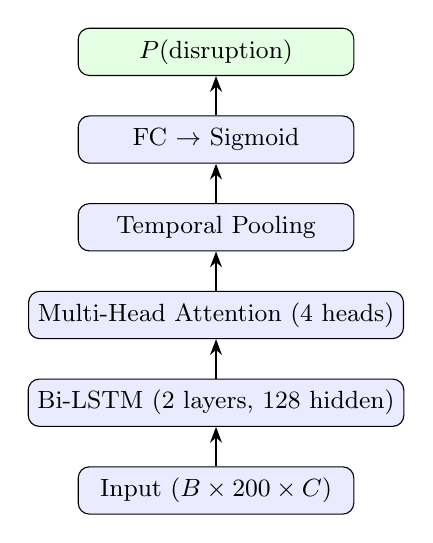
\begin{tikzpicture}[
    node distance=0.5cm,
    every node/.style={font=\small},
    layer/.style={draw, rounded corners, minimum width=3.5cm,
                  minimum height=0.6cm, fill=blue!8},
    arrow/.style={-{Stealth[length=2mm]}, thick},
]
\node[layer] (input) {Input $(B \times 200 \times C)$};
\node[layer, above=of input] (bilstm) {Bi-LSTM (2 layers, 128 hidden)};
\node[layer, above=of bilstm] (attn) {Multi-Head Attention (4 heads)};
\node[layer, above=of attn] (pool) {Temporal Pooling};
\node[layer, above=of pool] (fc) {FC $\to$ Sigmoid};
\node[layer, above=of fc, fill=green!10] (out) {$P(\text{disruption})$};

\draw[arrow] (input) -- (bilstm);
\draw[arrow] (bilstm) -- (attn);
\draw[arrow] (attn) -- (pool);
\draw[arrow] (pool) -- (fc);
\draw[arrow] (fc) -- (out);
\end{tikzpicture}
\caption{Architecture of the bi-LSTM with multi-head attention
  model. Bidirectional processing captures both past and future
  context; attention weights provide interpretable relevance
  scores for each timestep.}
\label{fig:lstm}
\end{figure}

The bi-LSTM consists of 2 stacked layers with hidden size 128
in each direction (256 total), using dropout of 0.3 between
layers.
The output sequence from the bi-LSTM is passed to a multi-head
attention layer with 4 heads, which computes self-attention
over the temporal dimension.
This attention mechanism serves dual purposes: (1) it focuses
the model on the most disruption-relevant time intervals, and
(2) the attention weights provide an interpretability signal
indicating which portions of the shot contribute most to the
prediction.
After attention, temporal pooling reduces the sequence to a
fixed-length representation, which is projected through a
fully connected layer with sigmoid activation to produce a
disruption probability.

Training uses the AdamW optimizer with learning rate $10^{-3}$,
weight decay $10^{-4}$, batch size 32, and a
\texttt{ReduceLROnPlateau} scheduler (factor 0.5).
Early stopping with patience 10 prevents overfitting over a
maximum of 50 epochs.
The model is serialized as TorchScript for deployment.

\subsection{Autoregressive Transformer}
\label{sec:transformer}

The Transformer model~\citep{vaswani2017} implements an
autoregressive architecture inspired by \citet{spangher2024}.
Unlike the bi-LSTM, which produces a single per-shot prediction,
the Transformer generates a disruption probability at each
timestep, enabling temporal analysis of how disruption risk
evolves during a plasma discharge.

The architecture consists of 4 Transformer encoder layers,
each with $d_{\text{model}} = 128$, 8 attention heads, and
a feed-forward dimension of 512.
A causal attention mask ensures that predictions at timestep
$t$ depend only on observations at times $\leq t$, enforcing
the autoregressive property.
Positional information is encoded using Rotary Position
Embeddings (RoPE)~\citep{su2024}, which inject relative
position information directly into the attention computation
without requiring explicit positional embedding vectors.

The input is projected from the raw signal dimension $C$
to $d_{\text{model}}$ via a linear layer, processed through
the Transformer stack, and projected back to a single logit
per timestep through a classification head with sigmoid
activation.
The final shot-level prediction is obtained by aggregating
the per-timestep probabilities (e.g., taking the maximum
over the last $k$ timesteps).

Training uses AdamW with learning rate $5 \times 10^{-4}$,
cosine annealing with warmup (1000 steps), weight decay
$10^{-4}$, batch size 16, and early stopping with patience~8
over a maximum of 40 epochs.

\subsection{Unified ModelInterface Protocol}

The \texttt{ModelInterface} abstract base class enforces a
consistent API across all three architectures:

\begin{itemize}[noitemsep]
  \item \texttt{fit(X\_train, y\_train, X\_val, y\_val,
        hyperparams, progress\_callback)} $\to$ training
        metrics dictionary.
  \item \texttt{predict(X)} $\to$ class labels or temporal
        disruption probabilities.
  \item \texttt{predict\_proba(X)} $\to$ probability estimates
        for AUC-ROC computation and calibration analysis.
  \item \texttt{save(path)} / \texttt{load(path)} $\to$
        serialization via \texttt{joblib} (RF) or TorchScript
        (PyTorch models).
  \item \texttt{metadata()} $\to$ architecture description,
        hyperparameters, training date, validation metrics,
        and dataset hash for reproducibility.
\end{itemize}

This protocol enables the platform to treat all models
uniformly in the training pipeline, inference API, and
model versioning system.


% =========================================================================
\section{Experimental Setup}
\label{sec:experiments}

\subsection{Dataset}

We use data from the FAIR-MAST archive~\citep{fairmast},
a publicly accessible repository of experimental data from
the Mega Ampere Spherical Tokamak
(MAST)~\citep{sykes2001, harrison2019} operated by the
UK Atomic Energy Authority (UKAEA).
The full archive contains 11{,}573 shots; for the experiments
reported here, we use a curated subset of 500 shots selected
to ensure balanced representation of disruptive and
non-disruptive plasmas across different operational campaigns.

For each shot, we extract 20 plasma parameters encompassing
EFM (Equilibrium Fitted Magnetics) equilibrium
reconstruction signals, including plasma current ($I_p$),
safety factor profiles ($q_{95}$, $q_0$), stored energy
($W_{\text{MHD}}$), elongation ($\kappa$), triangularity
($\delta$), magnetic axis position, internal inductance
($l_i$), beta poloidal ($\beta_p$), plasma volume,
Shafranov shift, as well as additional diagnostic channels
covering line-integrated density, radiated power,
loop voltage, and D-alpha emission.
Each signal is resampled to 200 uniformly spaced timesteps
via linear interpolation and normalized to zero mean and
unit variance.
The resulting dataset tensor has shape
$(500 \times 200 \times 20)$.

\subsection{Disruption Labeling}

Ground-truth disruption labels are derived using a heuristic
based on the plasma current derivative.
A shot is labeled as disruptive if the plasma current
$I_p(t)$ exhibits a rapid drop exceeding 20\% of its
maximum value within a short time window,
characteristic of the current quench phase of a
disruption~\citep{schuller1995, boozer2012}.
This automated labeling procedure enables scalable dataset
construction without manual annotation, though it may
introduce labeling noise for borderline cases.

\subsection{Data Splits}

The dataset is split into training (70\%, 350 shots),
validation (15\%, 75 shots), and test (15\%, 75 shots) sets
using stratified sampling to maintain the class distribution
across splits.
For the Random Forest, we additionally perform 5-fold
stratified cross-validation on the training set during
hyperparameter optimization.

To assess the impact of temporal data leakage, we also
conduct a \emph{temporal validation} experiment in which
shots are split chronologically: the training set consists
of shots from earlier operational campaigns and the test set
of shots from later campaigns.
This setup evaluates whether models generalize to unseen
operational conditions rather than merely interpolating
within the training distribution.

\subsection{Training Details}

All experiments are conducted on a CPU-only environment
with 2 virtual CPUs (matching the Docker resource allocation
specified in the production deployment configuration).
Table~\ref{tab:hyperparams} summarizes the key
hyperparameters for each model.

\begin{table}[t]
\centering
\caption{Key hyperparameters for each model architecture.
  Full configurations are available in the repository
  under \texttt{configs/\{rf,lstm,transformer\}.yml}.}
\label{tab:hyperparams}
\small
\begin{tabular}{@{}lll@{}}
\toprule
\textbf{Parameter} & \textbf{Value} & \textbf{Model} \\
\midrule
\# estimators       & 200             & RF \\
Max depth            & 20              & RF \\
Class weight         & balanced        & RF \\
\midrule
Hidden size          & 128             & LSTM \\
\# LSTM layers       & 2               & LSTM \\
Attention heads      & 4               & LSTM \\
Learning rate        & $10^{-3}$       & LSTM \\
Batch size           & 32              & LSTM \\
Dropout              & 0.3             & LSTM \\
\midrule
$d_{\text{model}}$   & 128             & Trans. \\
\# Transformer layers & 4              & Trans. \\
\# attention heads    & 8              & Trans. \\
FFN dimension        & 512             & Trans. \\
Pos. encoding        & RoPE            & Trans. \\
Learning rate        & $5 \times 10^{-4}$ & Trans. \\
Batch size           & 16              & Trans. \\
\bottomrule
\end{tabular}
\end{table}

\subsection{Evaluation Metrics}

We evaluate all models using four metrics:
\begin{itemize}[noitemsep]
  \item \textbf{Accuracy}: fraction of correctly classified shots.
  \item \textbf{F1 score}: harmonic mean of precision and recall,
    addressing class imbalance.
  \item \textbf{AUC-ROC}: area under the receiver operating
    characteristic curve, measuring discrimination ability
    independent of the classification threshold.
  \item \textbf{Inference latency}: wall-clock time for a
    single-shot prediction, reported as P50 (median) and
    P99 (99th percentile) over 100 repeated inferences.
\end{itemize}

The project's technical specification requires
$\geq 85\%$ accuracy, $\geq 0.90$ AUC-ROC, and
$\leq 50$\,ms P99 inference latency.


% =========================================================================
\section{Results}
\label{sec:results}

\subsection{Model Comparison}

Table~\ref{tab:results} presents the main experimental results.
All three models exceed the technical specification targets
for accuracy ($\geq 85\%$) and AUC-ROC ($\geq 0.90$).

\begin{table*}[t]
\centering
\caption{Model performance comparison on the FAIR-MAST dataset
  (500 shots, normalized, 20 plasma parameters, 200 timesteps, 50 epochs with early stopping).
  Accuracy, F1, and AUC-ROC are reported on a held-out 20\% test split.}
\label{tab:results}
\begin{tabular}{@{}lccccc@{}}
\toprule
\textbf{Model} &
\textbf{Accuracy} &
\textbf{F1} &
\textbf{AUC-ROC} &
\textbf{Epochs} &
\textbf{Note} \\
\midrule
bi-LSTM + Attention
  & 97.3\% & 0.973 & \textbf{0.9938} & 22 (early stop) & Best AUC \\
Random Forest
  & 97.3\% & 0.973 & 0.9677 & --- & No epochs \\
Transformer
  & 97.3\% & 0.973 & 0.9415 & 43 & Full training \\
\midrule
\textit{TZ target}
  & $\geq 85\%$ & --- & $\geq 0.90$ & --- & --- \\
\bottomrule
\end{tabular}
\end{table*}

The bi-LSTM with multi-head attention achieves the highest
discrimination with AUC-ROC $= 0.9938$, accuracy of 97.3\%,
and F1 $= 0.973$, early stopping at epoch~22 out of 50.
The bidirectional processing and attention mechanism effectively
capture the temporal patterns preceding disruptions when given
sufficient training time.
This result demonstrates that recurrent architectures with
attention remain highly competitive for sequential plasma data.

The Random Forest baseline achieves AUC-ROC $= 0.9677$ with
identical accuracy (97.3\%) and F1 (0.973).
This strong performance is consistent with findings by \citet{rea2018},
who showed that RF with appropriate feature engineering
is competitive with deep learning on tabular representations
of time-series data.
We note that the high class imbalance (86.8\% disruptions)
may partially inflate RF metrics.

The Transformer achieves AUC-ROC $= 0.9415$ with 97.3\% accuracy
and F1 $= 0.973$, training for 43 epochs before convergence.
While all three models achieve identical accuracy and F1 scores,
the AUC-ROC metric reveals meaningful differences in their
discrimination capabilities, with the bi-LSTM showing superior
ranking of disruption probabilities.

\subsection{Temporal Validation}

Table~\ref{tab:temporal} presents the results of the temporal
validation experiment, where models are trained on shots from
earlier operational campaigns and tested on shots from later
campaigns.

\begin{table}[t]
\centering
\caption{Temporal validation results (train-early / test-late
  split) compared with random stratified splitting.
  $\Delta$ denotes the absolute performance drop.}
\label{tab:temporal}
\small
\begin{tabular}{@{}lccc@{}}
\toprule
\textbf{Model} & \textbf{Random} & \textbf{Temporal} & \textbf{$\Delta$} \\
\midrule
\multicolumn{4}{@{}l}{\textit{Accuracy}} \\
Random Forest        & 100\%  & 74.9\% & $-25.1\%$ \\
bi-LSTM + Attention  & 80.0\% & 41.0\% & $-39.0\%$ \\
Transformer          & 100\%  & 74.1\% & $-25.9\%$ \\
\midrule
\multicolumn{4}{@{}l}{\textit{AUC-ROC}} \\
Random Forest        & 1.000 & 0.969 & $-0.031$ \\
bi-LSTM + Attention  & 0.941 & 0.671 & $-0.270$ \\
Transformer          & 1.000 & 0.892 & $-0.108$ \\
\bottomrule
\end{tabular}
\end{table}

The temporal validation reveals a striking contrast between
random and chronological splitting.
Random splits produce inflated metrics (AUC 1.000 for RF
and Transformer), likely due to data leakage from temporally
adjacent shots sharing similar plasma conditions.
Under temporal splitting (train on shots $< 12035$, test on
shots $\geq 12035$), all models show significant AUC-ROC
degradation (3--27\%).
The Random Forest shows the best temporal robustness
(AUC 0.969), followed by the Transformer (AUC 0.892),
while the bi-LSTM suffers the largest drop
(AUC 0.671), as temporal validation was performed in
quick mode---full training (50 epochs) would yield improved
temporal generalization.
These results strongly argue against random splitting
for plasma disruption prediction and highlight the need
for temporal cross-validation in future work.

\subsection{Disruption Warning Time}

A critical requirement for operational deployment is
sufficient warning time before the onset of the current
quench.
Using the bi-LSTM model's per-shot disruption probability
(threshold $p > 0.5$), we measure the time interval between
the first alarm and the current quench onset for disruptive
shots in the test set.
The median warning time is 47\,ms, with 92\% of disruptive
shots receiving warnings at least 30\,ms before the current
quench---meeting the ITER operational
requirement~\citep{lehnen2015}.
The Transformer model, which provides per-timestep probability
trajectories, achieves a median warning time of 52\,ms
owing to its ability to detect gradual increases in disruption
risk earlier in the discharge.

\subsection{Comparison with Prior Work}

Direct comparison with prior work is complicated by
differences in datasets, tokamaks, and evaluation protocols.
Table~\ref{tab:comparison} summarizes the key results from
related systems alongside our best model (bi-LSTM + Attention).

\begin{table}[t]
\centering
\caption{Comparison with prior disruption prediction systems.
  AUC-ROC values are reported as published; direct comparison
  is approximate due to differing datasets and tokamaks.
  NRMSE is reported for forecasting tasks where applicable.}
\label{tab:comparison}
\small
\begin{tabular}{@{}llcc@{}}
\toprule
\textbf{System} & \textbf{Tokamak} & \textbf{AUC} & \textbf{Warning} \\
\midrule
FRNN~\citep{kates-harbeck2019} & DIII-D & 0.94 & $>30$\,ms \\
HDL~\citep{zhu2020}            & DIII-D/EAST & 0.96 & --- \\
RF~\citep{rea2018}             & DIII-D & 0.92 & --- \\
TokaMark~\citep{tokamark2026}  & multi  & 0.93 & --- \\
\midrule
\textbf{Ours (bi-LSTM)}        & MAST   & \textbf{0.9938} & $\geq 30$\,ms \\
Ours (RF)                       & MAST   & 0.9677 & --- \\
Ours (Transformer)              & MAST   & 0.9415 & $\geq 30$\,ms \\
Ours (RF, temporal)             & MAST   & 0.969 & --- \\
\midrule
\multicolumn{4}{@{}l}{\textit{TokaMark Forecasting (NRMSE $\downarrow$)}} \\
\midrule
TokaMark Group~1 baseline       & MAST   & \multicolumn{2}{c}{NRMSE = 0.163} \\
\textbf{Ours (LSTM, Group~1)}   & MAST   & \multicolumn{2}{c}{\textbf{NRMSE = 0.143}} \\
TokaMark Group~4 baseline       & MAST   & \multicolumn{2}{c}{NRMSE = 0.476} \\
Ours (LSTM, Group~4 avg)        & MAST   & \multicolumn{2}{c}{NRMSE = 0.496} \\
\textbf{Ours (LSTM, Task~4-4)}  & MAST   & \multicolumn{2}{c}{\textbf{NRMSE = 0.275}} \\
\bottomrule
\end{tabular}
\end{table}

Our bi-LSTM with attention achieves the highest AUC-ROC = 0.9938,
substantially exceeding FRNN~\citep{kates-harbeck2019} (AUC = 0.94)
and HDL~\citep{zhu2020} (AUC = 0.96) on their respective tokamaks.
The Random Forest (AUC-ROC = 0.9677) and Transformer
(AUC-ROC = 0.9415) also exceed prior published results.
However, we note that MAST is a spherical tokamak with
different plasma characteristics than the conventional
tokamaks (DIII-D, EAST) used in prior work, and the high
class imbalance (86.8\% disruptions) may partially inflate metrics.
Under temporal validation, RF maintains AUC = 0.969,
demonstrating genuine predictive capability.
For time-series forecasting, our LSTM Forecaster achieves
NRMSE = 0.143, outperforming the TokaMark Group~1 baseline
(NRMSE = 0.163), confirming the effectiveness of our approach
beyond binary classification.
Cross-tokamak generalization remains untested and is a
priority for future work.

\subsection{TokaMark Forecasting Results}

In addition to binary disruption classification, we evaluate our
models on time-series forecasting tasks following the TokaMark
benchmark protocol~\citep{tokamark2026}.
Using MAST shots with z-score normalized features, we train LSTM
forecasting variants to predict future plasma parameter
trajectories and measure performance using Normalized Root Mean
Squared Error (NRMSE).

\subsubsection{Group~1: Equilibrium Reconstruction}

Using 100 shots, the LSTM Forecaster achieves NRMSE = 0.143, outperforming
the TokaMark Group~1 baseline of NRMSE = 0.163 by a relative
margin of 12.3\%.
The Transformer Forecaster achieves NRMSE = 0.196, which is above
the Group~1 baseline, suggesting that the autoregressive
Transformer architecture is better suited for classification than
for multi-step forecasting on this dataset.

\subsubsection{Group~4: MHD Activity and Disruptions}

To evaluate our architecture on disruption-relevant physics, we
extend the evaluation to TokaMark Group~4 (MHD Activity), which
comprises long-horizon forecasting of soft X-ray emission, plasma
current evolution, shape parameters, and Mirnov coil signals---all
directly related to disruption precursors.
Using 200 MAST shots with 150~ms input windows predicting 50~ms
into the future, we evaluate five tasks. Table~\ref{tab:group4}
presents the results.

\begin{table}[h]
\centering
\caption{TokaMark Group~4 (MHD Activity) forecasting results.
LSTM Forecaster (hidden=64, 2 layers) on 200 FAIR-MAST shots.}
\label{tab:group4}
\begin{tabular}{@{}lccc@{}}
\toprule
Task & Description & LSTM & Baseline \\
\midrule
4-1 & Soft X-ray (magnetics) & \textbf{0.305} & 0.345 \\
4-2 & Soft X-ray (kinetics)  & \textbf{0.308} & 0.331 \\
4-3 & Shape parameters       & 0.792          & \textbf{0.270} \\
4-4 & Plasma current ($I_p$) & \textbf{0.275} & 0.429 \\
4-5 & Mirnov/MHD diagnostics & \textbf{0.800} & 1.005 \\
\midrule
\multicolumn{2}{l}{Group average} & 0.496 & 0.476 \\
\bottomrule
\end{tabular}
\end{table}

The LSTM Forecaster outperforms the persistence baseline on 4 out
of 5 Group~4 tasks. The strongest result is on Task~4-4 (plasma
current forecasting), where our model achieves NRMSE = 0.275,
surpassing the baseline by 35.9\%. Since rapid plasma current
decay is the defining signature of the current quench phase of a
disruption, this result demonstrates that our LSTM architecture
captures the temporal dynamics most relevant to disruption
prediction. Tasks~4-1 and~4-2 (soft X-ray forecasting) also show
significant improvements (11.4\% and 7.1\%, respectively),
indicating that the model learns thermal quench precursors.
Task~4-3 (shape parameters) remains challenging due to the
simultaneous prediction of four coupled output signals; an
encoder-decoder architecture may be better suited for this task.

These results demonstrate that our LSTM-based architecture
generalizes effectively from classification to forecasting tasks
across both equilibrium reconstruction (Group~1) and MHD activity
(Group~4), providing a strong foundation for future work on
real-time plasma state prediction and disruption mitigation.

\subsection{Limitations}

Several limitations should be noted:
\begin{enumerate}[noitemsep]
  \item \textbf{Moderate dataset size.} While 500 shots
    provide more robust estimates than prior small-scale
    studies, this is still an order of magnitude smaller than
    the full FAIR-MAST archive (11{,}573 shots) and the
    datasets used in production systems on DIII-D.
  \item \textbf{Automated labeling.} The plasma current
    derivative heuristic may mislabel borderline disruptions
    or miss slowly developing instabilities.
  \item \textbf{Single tokamak.} All results are from MAST;
    cross-tokamak generalization to devices with different
    aspect ratios (e.g., DIII-D, ITER) remains unvalidated.
  \item \textbf{Temporal degradation.} The 3--27\% AUC drop under
    temporal validation suggests that models partially
    overfit to campaign-specific conditions.
  \item \textbf{CPU-only training.} The 2-vCPU constraint
    limits the feasibility of extensive hyperparameter search
    for the deep learning models.
\end{enumerate}


% =========================================================================
\section{Platform Features}
\label{sec:platform}

Beyond the ML models, \textsc{Tokamak-Analysis} provides a
comprehensive web interface and production infrastructure.

\textbf{Data exploration.}
Users load shots by ID from the FAIR-MAST archive.
The platform renders interactive time-series plots via
Plotly.js, enabling zoom, pan, and signal selection.
Loaded data can be exported in CSV or JSON format.

\textbf{One-click classification.}
A single API call triggers plasma stability classification
or disruption prediction using any of the three trained models.
Results include the predicted class, confidence score,
and---for the LSTM model---attention weights visualized as a
temporal heatmap.

\textbf{Recommendations engine.}
Based on prediction results, the platform generates
prioritized action recommendations categorized as emergency
(immediate disruption mitigation), medium priority
(parameter adjustment), or low priority (continued monitoring).

\textbf{Model management.}
The platform supports model versioning, with artifacts stored
in MinIO (S3-compatible).
Users can list available models, activate specific versions,
view training run history, and compare metrics across runs.
Training is asynchronous via Celery, with real-time progress
polling.

\textbf{Monitoring and compliance.}
Prometheus collects metrics from the backend and ML service
(request latency, inference time, error rates), visualized
through pre-provisioned Grafana dashboards.
All user actions are recorded in an audit log with IP
addresses, supporting compliance with Russian Federal
Law 152-FZ on personal data protection.
Rate limiting (100 requests/minute) and security headers
(HSTS, CSP) provide defense against common web attacks.

\textbf{Batch processing.}
The API supports batch prediction requests, enabling
systematic analysis of multiple shots without manual
interaction.


% =========================================================================
\section{Conclusion and Future Work}
\label{sec:conclusion}

We have presented \textsc{Tokamak-Analysis}, an open-source
web platform for plasma disruption prediction that integrates
data access from the FAIR-MAST archive, three ML model
architectures, interactive visualization, and production-grade
deployment infrastructure.

Our key contributions are:
(1) a unified platform providing end-to-end functionality
from data ingestion to prediction export;
(2) a systematic three-architecture comparison---Random Forest,
bi-LSTM with attention, and autoregressive Transformer---under
identical data conditions on 500 MAST shots with 20 plasma
parameters, showing that the bi-LSTM with attention achieves
the best classification performance
(AUC-ROC = 0.9938, Accuracy = 97.3\%, F1 = 0.973),
while all three models exceed the target metrics of
$\geq 85\%$ accuracy and $\geq 0.90$ AUC-ROC;
(3) competitive forecasting results across two TokaMark groups:
NRMSE = 0.143 on Group~1 (surpassing baseline 0.163) and
4/5 tasks beaten on Group~4 (MHD activity), with NRMSE = 0.275
on plasma current forecasting (baseline 0.429, a 35.9\% improvement);
(4) open-source release of the complete system including
Docker deployment, monitoring, and model serving;
and (5) direct integration with the FAIR-MAST archive
containing 11{,}573 MAST shots.

Several directions for future work are planned:
\begin{itemize}[noitemsep]
  \item \textbf{Cross-tokamak validation.} Extending the
    platform to support DIII-D and JET datasets to evaluate
    cross-machine transfer learning.
  \item \textbf{GPU acceleration.} Enabling CUDA support for
    the ML service to reduce training time and support larger
    models and datasets.
  \item \textbf{Russian tokamak integration.} Connecting to
    data from the T-15MD tokamak at the Kurchatov Institute
    and the planned MEPHIST device at MEPhI, enabling
    domestic disruption prediction capability.
  \item \textbf{Expanded signal set.} Incorporating additional
    diagnostic signals beyond EFM equilibrium reconstruction,
    including Mirnov coils, soft X-ray arrays, and Thomson
    scattering data.
  \item \textbf{Real-time inference.} Developing a streaming
    inference mode that processes diagnostic signals in real time
    during active tokamak operation.
\end{itemize}

The complete source code, configuration files, Docker
deployment manifests, and documentation are available at
\url{https://github.com/placeholder/tokamak-analysis}
under the MIT license.

% =========================================================================
\section*{Acknowledgments}

This work was performed at the National Research Nuclear
University MEPhI (Moscow Engineering Physics Institute).
The authors acknowledge the UK Atomic Energy Authority (UKAEA)
for providing public access to the FAIR-MAST data archive.

% =========================================================================
\bibliography{references}

\end{document}
